\begin{name}
	{Biên soạn: Thầy Duong Xuan Loi, Vinh Vo \& Phản biện: Thầy Vinh Vo, Duong Xuan Loi}
	{Đề thi giữa học kì 1 môn Toán THPT Ngô Gia Tự - Đắk Lắk, năm 2020 - 2021}
\end{name}
	\setcounter{ex}{0}\setcounter{bt}{0}
	\Opensolutionfile{ans}[ans/ans-2-GHK1-27-NgoGiaTu-Daklak-21]

\begin{ex}%[Thi giữa kì 1, Ngo Gia Tự - Đắk Lắk, 2021]%[Duong Xuan Loi, 12EX3-21]%[2D1Y2-2]
	Cho hàm số $y=f(x)$ liên tục trên $\mathbb{R}$ và có bảng biến thiên như sau
	\begin{center}
		
\begin{tikzpicture}
			\tkzTabInit[nocadre=false,lgt=1.2,espcl=2.5,deltacl=0.6]
			{$x$ /0.6, $f'(x)$ /0.6, $f(x)$ /2.5}
			{$-\infty$,$-1$,$2$,$+\infty$}
			\tkzTabLine{,+,$0$,-,$0$,+,}
			\tkzTabVar{-/$-\infty$,+/$3$,-/$0$,+/$+\infty$}
		\end{tikzpicture}
	\end{center}
	Hàm số đạt cực tiểu tại
	\choice
	{$x=-1$}
	{$y=0$}
	{\True $x=2$}
	{$y=3$}
	\loigiai{
		Từ bảng biến thiên suy ra hàm số đạt cực tiểu tại $x=2$.
	}
\end{ex}
\begin{ex}%[Thi giữa kì 1, Ngo Gia Tự - Đắk Lắk, 2021]%[Duong Xuan Loi, 12EX3-21]%[2D1Y1-2]
	Cho hàm số $y=f(x)$ có bảng biến thiên như sau
	\begin{center}
		
\begin{tikzpicture}
			\tkzTabInit[nocadre=false,lgt=1.2,espcl=2.5,deltacl=0.6]
			{$x$ /0.6,$f'(x)$ /0.6,$f(x)$ /2}
			{$-\infty$,$-\sqrt{2}$,$0$,$\sqrt{2}$,$+\infty$}
			\tkzTabLine{,-,$0$,+,$0$,-,$0$,+,}
			\tkzTabVar{+/$+\infty$, -/$-2$,+/$2$,-/$-2$,+/$+\infty$}
		\end{tikzpicture}
	\end{center}
	Hàm số $y=f(x)$ đồng biến trên khoảng nào dưới đây?
	\choice
	{$(-\infty;-2)$}
	{\True $\left(-\sqrt{2};0\right)$}
	{$(-2;2)$}
	{$(-2;+\infty)$}
	\loigiai{
		Từ bảng biến thiên suy ra hàm số đồng biến trên khoảng $\left(-\sqrt{2};0\right)$ và $\left(\sqrt{2};+\infty\right)$.
	}
\end{ex}
\begin{ex}%[Thi giữa kì 1, Ngo Gia Tự - Đắk Lắk, 2021]%[Duong Xuan Loi, 12EX3-21]%[2H1Y1-1]
	Hình nào sau đây là hình đa diện?
	\begin{center}
		\begin{tikzpicture}[scale=0.9,line join=round,line cap=round,font=\footnotesize,>=stealth]
			\path 
			(-0.2,0) coordinate (A)
			(-1.3,-1) coordinate (B)
			(-1.7,0.7) coordinate (C)
			(-1.25,2.1) coordinate (D)
			(-0.35,1.5) coordinate (E)
			($(A)+(2.1,0)$) coordinate (A')
			($(B)+(3,0)$) coordinate (B')	
			($(B')+(C)-(B)$) coordinate (C')
			($(B')+(D)-(B)$) coordinate (D')	
			($(B')+(E)-(B)$) coordinate (E')
			($(A')+(0.6,-0.6)$) coordinate (G)
			($(A')+(0.9,0.5)$) coordinate (H)	
			;
			\draw (B')--(B)--(C)--(D)--(D') (C)--(C') (B')--(G)--(H)--(E')--(D')--(C')--cycle;
			\draw[dashed] (B)--(A)--(E)--(D) (A)--(A')--(G)--(H)--(A') (E)--(E');
			\node at (0.7,-1.3)[]{Hình $1$};		
		\end{tikzpicture}
		\quad
		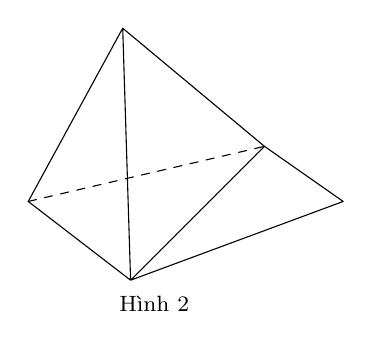
\begin{tikzpicture}[scale=1,line join=round,line cap=round,font=\footnotesize,>=stealth]
			\path 
			(0,0) coordinate (A)
			(1.3,-1) coordinate (B)
			(3,0.7) coordinate (C)
			(4,0) coordinate (D)
			(1.2,2.2) coordinate (S)		
			;
			\draw (A)--(B)--(C)--(S)--cycle (S)--(B)--(D)--(C);
			\draw[dashed] (A)--(C);
			\node at (1.6,-1.3)[]{Hình $2$};		
		\end{tikzpicture}
		\quad
		\begin{tikzpicture}[scale=0.8, font=\footnotesize, line join=round, line cap=round,>=stealth]
			\path 
			(0,0) coordinate (A')
			(1.9,-1) coordinate (B')
			(1,0.8) coordinate (C')
			(3.3,0) coordinate (D')
			(2.8,0.7) coordinate (E')		
			($(A')+(0,2.2)$) coordinate (A)
			($(A)+(B')-(A')$) coordinate (B)
			($(A)+(C')-(A')$) coordinate (C)
			($(A)+(D')-(A')$) coordinate (D)
			($(A)+(E')-(A')$) coordinate (E)
			;
			\draw (A)--(C)--(B)--(B')--(A')--cycle (A)--(B)--(D)--(D')--(B')
			(D)--(E)--(B);
			\draw[dashed] (A')--(C')--(C) (C')--(B') (E)--(E')--(B') (D')--(E');
			\node at (1.5,-1.3)[]{Hình $3$};		
		\end{tikzpicture}
		\quad
		\begin{tikzpicture}[scale=0.7,font=\footnotesize,line join=round,line cap=round,>=stealth]
			\coordinate (B) at (0,0);
			\coordinate (A) at (1,0.8);
			\coordinate (C) at (3,0);
			\coordinate (D) at ($(C)-(B)+(A)$);
			\coordinate (H) at ($(B)!1/3!(D)$);
			\coordinate (A') at ($(H)+(110:3.3)$);
			\coordinate (B') at ($(B)-(A)+(A')$);
			\coordinate (C') at ($(C)-(A)+(A')$);
			\coordinate (D') at ($(D)-(A)+(A')$);
			\coordinate (A1) at ($2*(B')-(A')$);
			\coordinate (C1) at ($2*(C')-(D')$);
			\coordinate (O) at (intersection of A1--C1 and B--B');
			\draw (O)--(B)--(C)--(D)--(D')--(A')--(B')--(C')--(D') (C)--(C')--(C1) (B')--(A1)--(C1);
			\draw[dashed] (B)--(A)--(D) (A')--(A) (O)--(B');
			\node at (1.5,-1)[]{Hình $4$};	
		\end{tikzpicture}
	\end{center}
	\choice
	{Hình $4$}
	{Hình $2$}
	{Hình $3$}
	{\True Hình $1$}
	\loigiai{
		\begin{itemize}
			\item Hình $1$ là hình đa diện.
			\item Hình $2$, hình $3$, hình $4$ không là hình đa diện vì có cạnh không là cạnh chung của đúng hai đa giác.
		\end{itemize}
	}
\end{ex}
\begin{ex}%[Thi giữa kì 1, Ngo Gia Tự - Đắk Lắk, 2021]%[Duong Xuan Loi, 12EX3-21]%[2D2Y4-2]
	Đạo hàm của hàm số $f(x)=\log_2\left(x^2+3x\right)$ là
	\choice
	{\True $\dfrac{2x+3}{\left(x^2+3x\right)\ln 2}$}
	{$\dfrac{2x+3}{x^2+3x}$}
	{$\dfrac{2x-3}{\left(x^2+3x\right)\ln 2}$}
	{$\dfrac{2x-3}{x^2+3x}$}
	\loigiai{
		Tập xác định $\mathscr{D}=(-\infty;-3)\cup(0;+\infty)$.\\
		$f'(x)=\dfrac{2x+3}{\left(x^2+3x\right)\ln 2}$.
	}
\end{ex}
\begin{ex}%[Thi giữa kì 1, Ngo Gia Tự - Đắk Lắk, 2021]%[Duong Xuan Loi, 12EX3-21]%[2H1Y3-2]
	Khối lăng trụ có diện tích đáy là $S$, chiều cao là $h$ thì thể tích của khối lăng trụ đó là
	\choice
	{$V=\dfrac{1}{3}Sh$}
	{$V=\dfrac{1}{6}Sh$}
	{\True $V=Sh$}
	{$V=\dfrac{1}{2}Sh$}
	\loigiai{
		Khối lăng trụ có diện tích đáy là $S$, chiều cao là $h$ thì thể tích $V=Sh$.
	}
\end{ex}
\begin{ex}%[Thi giữa kì 1, Ngo Gia Tự - Đắk Lắk, 2021]%[Duong Xuan Loi, 12EX3-21]%[2H1Y3-2]
	Cho hình chóp $S.ABCD$ có đáy là hình chữ nhật, $AB=a$, $AD=2a$. $SA$ vuông góc với mặt đáy, $SA=a$. Thể tích khối chóp là
	\choice
	{$V=\dfrac{a^3\sqrt{3}}{3}$}
	{$V=a^3\sqrt{3}$}
	{$V=\dfrac{1a^3}{3}$}
	{\True $V=\dfrac{2a^3}{3}$}
	\loigiai{
		\immini{
			Ta có $V=\dfrac{1}{3}\cdot SA\cdot S_{ABCD}=\dfrac{1}{3}\cdot a\cdot a\cdot 2a=\dfrac{2a^3}{3}$.
		}{
			\begin{tikzpicture}[scale=0.7, font=\footnotesize, line join=round, line cap=round,>=stealth]
				\path
				(0,0) coordinate (A)
				(-1.3,-1.6) coordinate (B)
				(2.5,-1.6)coordinate (C)
				($(A)+(C)-(B)$) coordinate (D)
				($(A)+(0,3)$) coordinate (S)
				;
				\draw (S)--(B)--(C)--(D)--cycle (S)--(C);
				\draw[dashed] (S)--(A)--(D) (A)--(B);	
				\foreach \p/\q in {S/90,A/-90,B/-90,C/-90,D/0}			
				\fill[black] (\p) circle (1.0pt)node[shift={(\q:2.5mm)}]{$\p$};	
				\tkzMarkRightAngles(S,A,B S,A,D)			
			\end{tikzpicture}
		}
	}
\end{ex}
\begin{ex}%[Thi giữa kì 1, Ngo Gia Tự - Đắk Lắk, 2021]%[Duong Xuan Loi, 12EX3-21]%[2H1Y3-2]
	Một lăng trụ tam giác đều có cạnh đáy bằng $2a$, cạnh bên bằng $a$ thể tích của khối lăng trụ đó bằng
	\choice
	{$\dfrac{4}{3} a^3$}
	{$\dfrac{1}{4} a^3\sqrt{3}$}
	{\True $a^3\sqrt{3}$}
	{$\dfrac{1}{2} a^3\sqrt{3}$}
	\loigiai{
		\immini{
			Ta có $V=AA'\cdot S_{ABC}=a\cdot \dfrac{(2a)^2\sqrt{3}}{4}=a^3\sqrt{3}$.
		}{
			\begin{tikzpicture}[scale=0.7, font=\footnotesize, line join=round, line cap=round,>=stealth]
				\path
				(0,0)coordinate (A)
				(1.1,-1.5)coordinate (B)
				(4,0)coordinate (C)
				($(A)+(0,3.2)$) coordinate (A')
				($(A')+(B)-(A)$)coordinate (B')
				($(A')+(C)-(A)$)coordinate (C')			
				;
				\draw (A)--(B)--(C)--(C')--(B')--(A')--cycle (A')--(C') (B)--(B');
				\draw[dashed] (A)--(C);	
				\foreach \p/\q in {A/180,B/-90,C/0,A'/180,B'/75,C'/0}
				\fill[black] (\p) circle (1.0pt)node[shift={(\q:3mm)}]{$\p$};
			\end{tikzpicture}
		}
	}
\end{ex}
\begin{ex}%[GHK1,THPT Ngô Gia Tự, 2020-2021]%[Vinh Vo, 12-EX3-2021]%[2H1Y2-2]
	Hình đa diện đều loại $ \{3;5\} $ là hình nào sau đây?
	\begin{center}
		\begin{tikzpicture}[scale=1, font=\footnotesize, line join=round, line cap=round, >=stealth]
			\tikzset{label style/.style={font=\footnotesize}}
			%	\tkzInit[xmin=0,xmax=2.6,ymin=-1.5,ymax=2]
			%	\tkzClip
			%	\tkzAxeXY
			\tkzDefPoints{0/-.8/D',2/-.8/C',0.6/0/A'}
			\coordinate (B') at ($(A')+(C')-(D')$);
			\tkzDefSquare(D',C')    \tkzGetPoints{C}{D}
			\tkzDefSquare(A',B')    \tkzGetPoints{B}{A}
			%	\tkzFillPolygon[color=violet!50!white, fill opacity=0.5](A,D,D',C',B',B)
			%	\tkzFillPolygon[color=violet!40!white, fill opacity=0.5](A,B,C,D)
			%	\tkzFillPolygon[color=violet!40!white, fill opacity=0.5](A',B',C',D')	
			\tkzDrawPolygon(A,B,B',C',D',D)
			\tkzDrawSegments(C,B C,D C,C')
			\tkzDrawSegments[dashed](A',A A',B' A',D')
			\draw (1.3,-1.2) node[] {\footnotesize Hình 1};
		\end{tikzpicture}
		\quad \quad
		\begin{tikzpicture}[scale=1, font=\footnotesize, line join=round, line cap=round, >=stealth]
			\tikzset{label style/.style={font=\footnotesize}}
			%	\tkzInit[xmin=0,xmax=3.5,ymin=-1.5,ymax=2]
			%	\tkzClip
			%	\tkzAxeXY
			\tkzDefPoints{0/0.2/A,2.5/0.2/B,1/0.8/D}
			\coordinate (C) at ($(D)+(B)-(A)$);
			\coordinate (I) at ($(A)!0.5!(C)$);
			\coordinate (M) at ($(I)+(0,1.5)$);
			\coordinate (N) at ($(I)-(0,1.4)$);
			%	\tkzFillPolygon[color=violet!30!white, fill opacity=0.5](M,A,N,C)
			\tkzDrawPolygon(M,A,B,C)
			\tkzDrawSegments(M,B N,A N,B N,C)
			\tkzDrawSegments[dashed](C,D A,D M,D N,D)
			\draw (1.75,-1.2) node[] {\footnotesize Hình 2};
		\end{tikzpicture}
		\quad \quad 
		
\begin{tikzpicture}[scale=1, font=\footnotesize, line join=round, line cap=round, >=stealth]
			\tikzset{label style/.style={font=\footnotesize}}
			%	\tkzInit[xmin=0,xmax=3,ymin=-1.5,ymax=2]
			%	\tkzClip
			%	\tkzAxeXY
			\tkzDefPoints{1.5/0.56/O,1.5/-0.9/A,1.5/-0.3/B}
			\foreach \x / \i in {36/1, 72/2, 108/3, 144/4, 180/5, 216/6, 256/7, 288/8, 324/9}
			{
				\tkzDefPointBy[rotation = center O angle \x](A)    \tkzGetPoint{A\i}
				\tkzDefPointBy[rotation = center O angle \x](B)    \tkzGetPoint{B\i}
			}
			%	\tkzFillPolygon[color=violet!30!white, fill opacity=0.5](A,A1,A2,A3,A4,A5,A6,A7,A8,A9)
			\tkzDrawPolygon(A,A1,A2,A3,A4,A5,A6,A7,A8,A9)
			\tkzDrawPolygon[dashed](B,B2,B4,B6,B8)
			\tkzDrawPolygon(B1,B3,B5,B7,B9)
			\tkzDrawSegments(B1,A1 B3,A3 B5,A5 B7,A7 B9,A9)
			\tkzDrawSegments[dashed](B,A B2,A2 B4,A4 B6,A6 B8,A8)
			\draw (1.5,-1.2) node[] {\footnotesize Hình 3};
		\end{tikzpicture}
		\quad \quad
		
\begin{tikzpicture}[scale=1, font=\footnotesize, line join=round, line cap=round, >=stealth]
			\tikzset{label style/.style={font=\footnotesize}}
			%	\tkzInit[xmin=0,xmax=3,ymin=-1.5,ymax=2]
			%	\tkzClip
			%	\tkzAxeXY
			\tkzDefPoints{1.5/0.56/O,1.5/-0.9/A,1.5/-0.3/B}
			\foreach \x / \i in {60/1, 120/2, 180/3, 240/4, 300/5}
			{
				\tkzDefPointBy[rotation = center O angle \x](A)    \tkzGetPoint{A\i}
			}
			%	\tkzFillPolygon[color=violet!30!white, fill opacity=0.5](A,A1,A2,A3,A4,A5)
			\tkzDrawPolygon(A,A1,A2,A3,A4,A5)
			\tkzDefPointBy[rotation = center O angle -40](B)    \tkzGetPoint{B0}
			\foreach \x / \i in {60/1, 120/2, 180/3, 240/4, 300/5}
			{
				\tkzDefPointBy[rotation = center O angle \x](B0)    \tkzGetPoint{B\i}
			}
			\tkzDrawPolygon(B0,B2,B4)
			\tkzDrawPolygon[dashed](B1,B3,B5)
			\tkzDrawSegments(B0,A B0,B9 B2,A B2,A1 B2,A2 B4,A3 B4,A2 B4,A4 B0,A5 B0,A4)
			\tkzDrawSegments[dashed](B1,A B1,A1 B3,A1 B3,A2 B3,A3 B5,A3 B5,A4 B5,A5 B1,A5)
			\draw (1.5,-1.2) node[] {\footnotesize Hình 4};
		\end{tikzpicture}
	\end{center}
	\choice
	{Hình $ 3 $}
	{Hình $ 2 $}
	{\True Hình $ 4 $}
	{Hình $ 1 $}
	\loigiai{
		Hình $4$ là hình đa diện đều loại $ \{3;5\} $.
	}
\end{ex}
\begin{ex}%[GHK1,THPT Ngô Gia Tự, 2020-2021]%[Vinh Vo, 12-EX3-2021]%[2D1Y5-3]
	Cho hàm số $ y = f(x) $ có bảng biến thiên như hình vẽ.
	\begin{center}
		
\begin{tikzpicture}
			%	\tikzset{double style/.append style = {double distance=2pt}}
			\tkzTabInit[lgt=1.2,espcl=2] % tùy chọn
			{$x$/0.6, $y'$/0.7, $y$/2} % cột đầu tiên
			{$-\infty$, $-1$, $3$,  $+\infty$} % hàng 1 cột 2
			\tkzTabLine{,+,0,-,0,+,} % hàng 2 cột 2
			\tkzTabVar{-/ $-\infty$, +/ $4$, -/ $-2$, +/ $+\infty$} % hàng 3 cột 2
		\end{tikzpicture}
	\end{center}
	Số nghiệm của phương trình $ f(x) = 1 $ là	
	\choice
	{$ 0 $}
	{$ 2 $}
	{$ 1 $}
	{\True $ 3 $}
	\loigiai{
		Từ bảng biến thiên, ta thấy $ f(x) = 1 $ có $ 3 $ nghiệm.	
	}
\end{ex}
\begin{ex}%[GHK1,THPT Ngô Gia Tự, 2020-2021]%[Vinh Vo, 12-EX3-2021]%[2D1Y4-1]
	Tiệm cận đứng và tiệm cận ngang của đồ thị hàm số $ y = \dfrac{3x - 1}{x + 1} $ lần lượt là
	\choice
	{$ x = \dfrac{1}{3}$; $y = 3 $}
	{$ y = - 1$; $x = 3 $}
	{$ y = 2$; $x = - 1 $}
	{\True $ x = - 1$; $y = 3 $}
	\loigiai{
		Ta có $ \heva{& \lim \limits_{x \to - \infty}  y = 3 \\ & \lim \limits_{x \to + \infty}  y = 3} \Rightarrow y = 3$ là tiệm cận ngang của đồ thị hàm số.\\
		Ta có $ \heva{& \lim \limits_{x \to - 1^{-}}  y = +\infty \\ & \lim \limits_{x \to - 1^{+} }  y = - \infty } \Rightarrow x = - 1$ là tiệm cận đứng của đồ thị hàm số.
	}
\end{ex}
\begin{ex}%[GHK1,THPT Ngô Gia Tự, 2020-2021]%[Vinh Vo, 12-EX3-2021]%[2H1Y1-2]
	Hình lục diện đều có bao nhiêu cạnh?
	\choice
	{$ 6 $ cạnh}
	{\True $ 12 $ cạnh}
	{$ 8 $ cạnh}
	{$ 20 $ cạnh}
	\loigiai{
		Hình lục diện đều là hình lập phương. Hình lập phương có $ 12 $ cạnh.
	}
\end{ex}
\begin{ex}%[GHK1,THPT Ngô Gia Tự, 2020-2021]%[Vinh Vo, 12-EX3-2021]%[2H1Y3-2]
	Khối chóp có diện tích đáy là $ B $, chiều cao $ h $ thì thể tích khối chóp là
	\choice
	{$ V = Bh $}
	{$ V = \dfrac{1}{2}Bh $}
	{\True $ V = \dfrac{1}{3}Bh $}
	{$ V = \dfrac{1}{4}Bh $}
	\loigiai{
		Thể tích khối chóp $ V = \dfrac{1}{3}Bh $.
	}
\end{ex}
\begin{ex}%[GHK1,THPT Ngô Gia Tự, 2020-2021]%[Vinh Vo, 12-EX3-2021]%[2H1Y3-2]
	Cho hình chóp $ S.ABC  $ có đáy là tam giác vuông cân tại $ A $, $ AB = a $. $ SA $ vuông góc với mặt đáy và $ SA = 2a $. Thể tích khối chóp là
	\choice
	{$ V = \dfrac{1}{12}a^3 \sqrt{3} $}
	{$ V = \dfrac{1}{6}a^3 \sqrt{3} $}
	{$ V = \dfrac{1}{6}a^3  $}
	{\True $ V = \dfrac{1}{3}a^3  $}
	\loigiai{
		\immini{
			Ta có $ S_{\triangle ABC} = \dfrac{1}{2} a^2 $.\\
			Thể tích $ V_{S.ABC} = \dfrac{1}{3} SA \cdot S_{\triangle ABC} = \dfrac{1}{3}a^3$.
		}{
			\begin{tikzpicture}[scale=0.7, font=\footnotesize, line join=round, line cap=round,>=stealth]
				\path
				(0,0) coordinate (A)
				(1.2,-1.5) coordinate (B)
				(4,0) coordinate (C)
				($(A)+(0,3.3)$) coordinate (S)	
				;
				\draw (S)--(A)--(B)--(C)--cycle (S)--(B);	
				\draw[dashed] (A)--(C);	
				\foreach \p/\q in {S/90,A/180,B/-90,C/0}
				\fill[black] (\p) circle (1.0pt) ($(\p)+(\q:2.5mm)$) node{$\p$};
				\tkzMarkRightAngles(B,A,C)
			\end{tikzpicture}
		}
	}
\end{ex}
\begin{ex}%[GHK1,THPT Ngô Gia Tự, 2020-2021]%[Vinh Vo, 12-EX3-2021]%[1H3Y4-2]
	Cho lăng trụ đều $ ABCD.A'B'C'D' $. Gọi $ O $ là tâm của đa giác đáy $ ABCD $.	Đường cao của lăng trụ là
	\choice
	{$ A'B $}
	{\True $ AA' $}
	{$ A'C $}
	{$ A'O $}
	\loigiai{
		Đường cao của hình lăng trụ đều là $ 1 $ cạnh bên bất kì.	
	}
\end{ex}
\begin{ex}%[GHK1,THPT Ngô Gia Tự, 2020-2021]%[Vinh Vo, 12-EX3-2021]%[2D2Y4-2]
	Đạo hàm của hàm số $ f(x) = 5^{ x^2 - 5x } $ là
	\choice
	{\True $ (2x - 5)5^{x^2 - 5x} \ln 5 $}
	{$ \left ( x^2 - 5x \right )5^{x^2 - 5x} $}
	{$ 5^{x^2 - 5x} \ln 5$}
	{$ (2x - 5) 5^{x^2 - 5x} $}
	\loigiai{
		Ta có $ f'(x) = \left ( x^2 - 5x \right )'\cdot 5^{x^2 - 5x} \ln 5 = (2x - 5)\cdot 5^{x^2 - 5x } \ln 5$.
	}
\end{ex}
\begin{ex}%[GHK1,THPT Ngô Gia Tự, 2020-2021]%[Vinh Vo, 12-EX3-2021]%[2D2Y4-1]
	Tập xác định của hàm số $ f(x) = \log_3 \left ( x^2 - 2x \right ) $ là
	\choice
	{$ \mathscr{D} = (-\infty; 0] \cup [2; + \infty) $}
	{$ \mathscr{D} = [0;2] $}
	{\True $ \mathscr{D} = (-\infty; 0) \cup (2; + \infty) $}
	{$ \mathscr{D} = (0;2) $}
	\loigiai{
		Hàm số $ f(x) $ có nghĩa $ \Leftrightarrow x^2 - 2x > 0 \Leftrightarrow x< 0 \lor x > 2 $.
	}
\end{ex}
\begin{ex}%[Thi giữa kì 1, Ngo Gia Tự - Đắk Lắk, 2021]%[Duong Xuan Loi, 12EX3-21]%[2H1B3-2]
	Cho hình chóp $S.ABC$ có đáy $ABC$ là tam giác vuông cân tại $B$ với $AC=2a$ biết $SA$ vuông góc với đáy $(ABC)$ và $SB$ hợp với mặt đáy một góc $60^{\circ}$. Tính thể tích hình chóp.
	\choice
	{$\dfrac{a^3\sqrt{6}}{6} $}
	{\True $\dfrac{a^3\sqrt{6}}{3}$}
	{$a^3\sqrt{6}$}
	{$\dfrac{a^3\sqrt{6}}{4}$}
	\loigiai{
		\immini{
			Ta giác $ABC$ vuông cân tại $B$ nên $2AB^2=AC^2\Rightarrow AB=a\sqrt{2}$.\\
			Hình chiếu vuông góc của $SB$ trên mặt phẳng $(ABC)$ là $AB$ do đó
			$60^{\circ}=(SB,(ABC))=(SB,AB)=\widehat{SBA}$.\\
			Tam giác $SAB$ vuông tại $A$, ta có 
			$$SA=AB\cdot\tan \widehat{SBA}=a\sqrt{2}\cdot\tan60^{\circ}=a\sqrt{6}.$$
			Vậy $V_{S.ABC}=\dfrac{1}{6}\cdot SA\cdot AB\cdot AC=\dfrac{1}{6}\cdot a\sqrt{6}\cdot a\sqrt{2}\cdot a\sqrt{2}=\dfrac{a^3\sqrt{6}}{3}$.
		}{
			\begin{tikzpicture}[scale=1, font=\footnotesize, line join=round, line cap=round,>=stealth]
				\path
				(0,0) coordinate (A)
				(1.2,-1.5) coordinate (B)
				(4,0) coordinate (C)
				($(A)+(0,3.3)$) coordinate (S)
				($(S)!0.5!(C)$) coordinate (I)
				;
				\draw (S)--(A)--(B)--(C)--cycle (S)--(B);	
				\draw[dashed] (A)--(C);	
				\foreach \p/\q in {S/90,A/180,B/-90,C/0}					
				\fill[black] (\p)node[shift={(\q:3mm)}]{$\p$} circle (1.0pt);
				\tkzMarkRightAngles(A,B,C S,A,B S,A,C)
				\tkzMarkAngles[size=0.7cm](S,B,A)									
			\end{tikzpicture}
		}		
	}
\end{ex}
\begin{ex}%[Thi giữa kì 1, Ngo Gia Tự - Đắk Lắk, 2021]%[Duong Xuan Loi, 12EX3-21]%[1H3B5-3]
	Cho hình chóp $S.ABC$ đáy là tam giác vuông tại $A$, $AB=a$, $BC=a\sqrt{3}$. $SA$ vuông góc với mặt đáy, $SA=a$. Khi đó khoảng cách từ $A$ đến mp$(SBC)$ bằng
	\choice
	{$\dfrac{a\sqrt{21}}{6}$}
	{\True $\dfrac{a\sqrt{10}}{5}$}
	{$\dfrac{a\sqrt{21}}{7}$}
	{$\dfrac{a\sqrt{10}}{3}$}
	\loigiai{
		\immini{
			Tam giác $ABC$ vuông tại $A$ nên $AC=\sqrt{BC^2-AB^2}=a\sqrt{2}$.\\
			Gọi $K$, $H$ lần lượt là hình chiếu vuông góc của $A$ trên $BC$, $SK$.\\
			Ta có $\heva{& AK\perp BC \\ & SA\perp BC}\Rightarrow BC\perp (SAH)\Rightarrow BC\perp AH$.\\
			$\heva{& BC\perp AH \\ & SK\perp AH}\Rightarrow AH\perp (SBC)$, do đó $\mathrm{d}\left(H,(SBC)\right)=AH$.\\
			Ta lại có $AH$, $AK$ lần lượt là đường cao của hai tam giác vuông $SAK$, $ABC$, nên
			$$\dfrac{1}{AH^2}=\dfrac{1}{AS^2}+\dfrac{1}{AK^2}=\dfrac{1}{AS^2}+\dfrac{1}{AB^2}+\dfrac{1}{AC^2}=\dfrac{1}{a^2}+\dfrac{1}{a^2}+\dfrac{1}{2a^2}\Rightarrow AH=\dfrac{a\sqrt{10}}{5}.$$
		}{
			\begin{tikzpicture}[scale=1, font=\footnotesize, line join=round, line cap=round,>=stealth]
				\path
				(0,0) coordinate (A)
				(1.2,-1.5) coordinate (B)
				(4,0) coordinate (C)
				($(A)+(0,3.3)$) coordinate (S)				
				($(B)!0.3!(C)$) coordinate (K)
				($(S)!0.6!(K)$) coordinate (H)
				;
				\draw (S)--(A)--(B)--(C)--cycle (K)--(S)--(B);	
				\draw[dashed] (K)--(A)--(C) (A)--(H);	
				\foreach \p/\q in {S/90,A/180,B/-90,C/0,K/-40,H/20}					
				\fill[black] (\p)node[shift={(\q:3mm)}]{$\p$} circle (1.0pt);
				\tkzMarkRightAngles(B,A,C A,K,B A,H,S)				
			\end{tikzpicture}
		}
	}
\end{ex}
\begin{ex}%[Thi giữa kì 1, Ngo Gia Tự - Đắk Lắk, 2021]%[Duong Xuan Loi, 12EX3-21]%[2D1B5-1]
	\immini{
		Xác định $a$, $b$, $c$ để hàm số $y=\dfrac{ax-1}{bx+c}$ có đồ thị như hình vẽ bên. Chọn đáp án đúng?
		\choice
		{\True $a=2$, $b=1$, $c=-1$}
		{$a=2$, $b=-1$, $c=1$}
		{$a=2$, $b=1$, $c=1$}
		{$a=2$, $b=2$, $c=-1$}
	}{
		\begin{tikzpicture}[scale=0.5, font=\footnotesize, line join=round, line cap=round,>=stealth]
			\def\a{2} \def\b{-1} \def\c{1} \def\d{-1} % Hệ số
			\def\xmin{-3.5} \def\xmax{5}
			\def\ymin{-3} \def\ymax{5}			
			\draw[->] (\xmin,0)--(\xmax,0) node [below]{$x$};
			\draw[->] (0,\ymin)--(0,\ymax) node [left]{$y$};
			\node at (0,0) [below left]{$O$};
			\clip (\xmin+0.1,\ymin+0.1) rectangle (\xmax-0.1,\ymax-0.1);
			\draw[smooth,samples=300,domain=\xmin:(-\d/\c-0.1)] plot(\x,{(\a*(\x)+\b)/(\c*(\x)+\d)});
			\draw[smooth,samples=300,domain=(-\d/\c+0.1:\xmax)] plot(\x,{(\a*(\x)+\b)/(\c*(\x)+\d)});
			\draw[dashed] (-\d/\c,\ymin)--(-\d/\c,\ymax);
			\draw[dashed] (\xmin,\a/\c)--(\xmax,\a/\c);
			\fill (0,0) circle (1.0pt) (1,0) circle (1.0pt)node[below right]{$1$} (0,2) circle (1.0pt)node[above right]{$2$} (0,1) circle (1.0pt)node[above right]{$1$};
		\end{tikzpicture}
	}
	\loigiai{
		Đồ thị hàm số đi qua điểm $(0;1)\Rightarrow c=-1$.\\
		Đồ thị hàm số có tiệm cận đứng $x=1\Rightarrow -\dfrac{c}{b}=1\Rightarrow b=1$.\\
		Đồ thị hàm số có tiệm cận ngang $y=2\Rightarrow \dfrac{a}{b}=2\Rightarrow a=2$.\\
	}
\end{ex}
\begin{ex}%[Thi giữa kì 1, Ngo Gia Tự - Đắk Lắk, 2021]%[Duong Xuan Loi, 12EX3-21]%[2D2B4-3]
	Cho hàm số $y=f(x)$ liên tục trên $\mathbb{R}$ và có bảng biến thiên như sau
	\begin{center}
		
\begin{tikzpicture}
			\tkzTabInit[nocadre=false,lgt=1.2,espcl=2.5,deltacl=0.6]
			{$x$ /0.6,$f'(x)$ /0.6,$f(x)$ /2}
			{$-\infty$,$-2$,$0$,$3$,$+\infty$}
			\tkzTabLine{,+,$0$,-,$0$,+,$0$,-,}
			\tkzTabVar{-/$-\infty$, +/$-1$,-/$-3$,+/$2$,-/$-\infty$}
		\end{tikzpicture}
	\end{center}
	Hàm số $y=\ln (f(x))$ có tất cả bao nhiêu điểm cực đại?
	\choice
	{\True $1$}
	{$2$}
	{$0$}
	{$3$}
	\loigiai{
		Xét $f(x)=0\Leftrightarrow \hoac{& x=a &\text{ với } 0<a<3\\ & x=b &\text{ với } b>3.}$\\
		Hàm số $y=\ln (f(x))$ xác định trên khoảng $(a;b)$.\\
		$y'=\dfrac{f'(x)}{f(x)}$, $y'=0\Leftrightarrow f'(x)=0\Leftrightarrow x=3\in(a;b)$.\\
		\begin{center}
			
\begin{tikzpicture}
				\tkzTabInit[nocadre=false,lgt=1,espcl=2.5,deltacl=0.6]
				{$x$ /0.6, $y'$ /0.6, $y$ /2.1}
				{$a$,$3$,$b$}
				\tkzTabLine{,+,$0$,-,}
				\tkzTabVar{-/$-\infty$, +/$\ln 2$,-/$-\infty$}
			\end{tikzpicture}
		\end{center}
		Vậy hàm số $y=\ln (f(x))$ có $1$ điểm cực đại.
	}
\end{ex}
\begin{ex}%[Thi giữa kì 1, Ngo Gia Tự - Đắk Lắk, 2021]%[Duong Xuan Loi, 12EX3-21]%[2D1B5-2]
	Cho hàm số $y=f(x)$ liên tục trên $[-2;4]$ và có bảng biến thiên như sau
	\begin{center}
		
\begin{tikzpicture}
			\tkzTabInit[nocadre=false,lgt=1.2,espcl=2.5,deltacl=0.6]
			{$x$ /0.6, $f(x)$ /2.5}
			{$-2$,$-1$,$0$,$4$}			
			\tkzTabVar{-/$-3$,+/$1$,-/$-2$,+/$2$}
		\end{tikzpicture}
	\end{center}
	Gọi $M$, $m$ lần lượt là giá trị lớn nhất, giá trị nhỏ nhất của hàm số $y=|f(x)|$ trên đoạn $[-2;4]$. Tính $M^2-m^2$.
	\choice
	{\True $9$}
	{$8$}
	{$3$}
	{$5$}
	\loigiai{
		Từ bảng biến thiên suy ra $f(x)=0\Leftrightarrow \hoac{& x=x_1&\text{ với } -2<x_1<-1\\ & x=x_2&\text{ với } -1<x_2<0\\&x=x_3&\text{ với } 0<x_3<4.}$\\
		Ta có bảng biến thiên của hàm số $y=|f(x)|$
		\begin{center}
			
\begin{tikzpicture}
				\tkzTabInit[nocadre=false,lgt=1.3,espcl=2.1,deltacl=0.6]
				{$x$ /0.6, $|f(x)|$ /2.5}
				{$-2$,$x_1$,$-1$,$x_2$,$0$,$x_3$,$4$}			
				\tkzTabVar{+/$3$,-/$0$,+/$1$,-/$0$,+/$2$,-/$0$,+/$2$}
			\end{tikzpicture}
		\end{center}
		Từ bảng biến thiên, ta có\\	
		$M=\max\limits_{[-2;4]} |f(x)|=|f(-2)|=3$, $m=\min\limits_{[-2;4]} |f(x)| =|f(x_1)|=|f(x_2)|=|f(x_3)|=0$.\\
		Vậy $M^2-m^2=9$.
	}
\end{ex}
\begin{ex}%[Thi giữa kì 1, Ngo Gia Tự - Đắk Lắk, 2021]%[Duong Xuan Loi, 12EX3-21]%[2D2B3-1]
	Cho $\log_3 5=a$; $\log_3 6=b$; $\log_3 22=c$. Tính $P=\log_3\left(\dfrac{90}{11}\right)$ theo $a$, $b$, $c$ là
	\choice
	{$P=2a+b+c$}
	{$P=2a+b-c$}
	{$P=a-2b+c$}
	{\True $P=a+2b-c$}
	\loigiai{
		Ta có 
			\begin{eqnarray*}
				P&=&\log_3\left(\dfrac{90}{11}\right)=\log_3 90-\log_3 11\\
				&=&\log_3(3\cdot5\cdot6)-\log_3\dfrac{22\cdot3}{6}\\
				&=&1+\log_35+\log_36-\left(\log_322+1-\log_36\right)\\
				&=&\log_35+2\log_36-\log_322=a+2b-c.
			\end{eqnarray*}		
	}
\end{ex}
\begin{ex}%[Thi giữa kì 1, Ngo Gia Tự - Đắk Lắk, 2021]%[Duong Xuan Loi, 12EX3-21]%[2D1B3-1]
	Tìm giá trị nhỏ nhất của hàm số $y=x^3-6x^2+2$ trên đoạn $[-1;2]$.
	\choice
	{\True $-14$}
	{$-5$}
	{$2$}
	{$-30$}
	\loigiai{
		$y'=3x^2-12x$, $y'=0\Leftrightarrow\hoac{& x=4\notin [-1;2] \\ & x=0\in [-1;2].}$\\
		Mà $y(-1)=-5$, $y(0)=2$, $y(2)=-14$.\\
		Vậy $\min\limits_{[-1;2]} y=y(2)=-14$.		
	}
\end{ex}
\begin{ex}%[GHK1,THPT Ngô Gia Tự, 2020-2021]%[Vinh Vo, 12-EX3-2021]%[2H1B3-2]
	Cho hình chóp $ S.ABC $ có đáy là tam giác đều cạnh bằng $ a $, hình chiếu vuông góc $ S $ lên mặt đáy trùng với trung điểm $ M $ của cạnh $ BC $ và $ SA $ hợp với đáy một góc $ 45^{\circ} $. Thể tích khối chóp. 
	\choice
	{$ \dfrac{1}{6}a^3 \sqrt{3} $} 
	{\True $ \dfrac{1}{8}a^3 $}
	{$ \dfrac{1}{12}a^3 $}
	{$ \dfrac{1}{8}a^3 \sqrt{3} $}
	\loigiai{
		\immini{
			Ta có $ \triangle SMA $ vuông cân tại $ M \Rightarrow SM = AM = \dfrac{ \sqrt{3}a }{2}$.\\
			Ta có $ S_{\triangle ABC} = \dfrac{ \sqrt{3}a^2 }{4} $.\\
			Vậy $ V_{S.ABC} = \dfrac{1}{3} SM \cdot S_{\triangle ABC} = \dfrac{1}{8}a^3 $.
		}{
			\begin{tikzpicture}
				\tkzDefPoint(0,0){B}
				\tkzDefShiftPoint[B](0:3){A}
				\tkzDefShiftPoint[B](-20:1.5){C}
				\coordinate (M) at ($(C)!0.5!(B)$);
				\tkzDefShiftPoint[M](90:2.3){S}
				\tkzDrawSegments(S,B B,C C,S S,M C,A S,A)
				\tkzDrawSegments[dashed](A,M B,A)
				\tkzDrawPoints[fill = black](A,B,C,M,S)
				\tkzLabelPoints[below](A,B,C,M)
				\tkzLabelPoints[above](S)
			\end{tikzpicture}
		}		
	}
\end{ex}
\begin{ex}%[GHK1,THPT Ngô Gia Tự, 2020-2021]%[Vinh Vo, 12-EX3-2021]%[2D1B1-1]
	Hàm số $ y = x^3 - 3x^2 + 2 $ nghịch biến trên khoảng nào dưới đây?
	\choice
	{$ (- \infty; 2) $}
	{$ (-\infty; 0) $ và $ (2; + \infty) $}
	{$ (-2; 2) $}
	{\True $ (0;2) $}
	\loigiai{
		Ta có $ y' = 3x^2 - 6x $, $ y' = 0 \Leftrightarrow \hoac{&x = 0 \\ & x = 2} $. Ta có bảng biến thiên \begin{center}
			
\begin{tikzpicture}
				%	\tikzset{double style/.append style = {double distance=2pt}}
				\tkzTabInit[lgt=1.2,espcl=2] % tùy chọn
				{$x$/0.6, $y'$/0.7, $y$/2} % cột đầu tiên
				{$-\infty$, $0$, $2$,  $+\infty$} % hàng 1 cột 2
				\tkzTabLine{,+,0,-,0,+,} % hàng 2 cột 2
				\tkzTabVar{-/ , +/ , -/ , +/ } % hàng 3 cột 2
			\end{tikzpicture}
		\end{center}
		Từ bảng biến thiên, ta thấy hàm số nghịch biến trên $ (0;2) $.	
	}
\end{ex}

\begin{ex}%[GHK1,THPT Ngô Gia Tự, 2020-2021]%[Vinh Vo, 12-EX3-2021]%[2D1B2-2]
	\immini{
		Cho hàm số $ y = f(x) $ có đạo hàm $ f'(x) $ trên $ \mathbb{R} $. Đồ thị hàm số $ y = f'(x) $ như hình vẽ. Hàm số $ y = f(x) $ có bao nhiêu điểm cực tiểu?
		\choice
		{\True $ 1 $}
		{$ 4 $}
		{ $ 2 $}
		{$ 3 $}
	}{
		\begin{tikzpicture}[line cap=round,line join=round,x=1.0cm,y=1.0cm,>=stealth,scale=1.3, font = \footnotesize]
			\draw[-> ] (-1,0) -- (3.5,0)node[below] {$x$};
			\draw[-> ] (0,-1.8) -- (0,1)node[left] {$y$};
			\draw(-0.1,0) node[above left=-0.1] { $O$};
			\clip (-1,-1.8) rectangle (3.5,1);
			\draw [samples=100, domain=-0.5:3.3] plot (\x, {  (\x)*(\x -1)*(\x - 1)*(\x - 3)*.5   });
			\draw[dashed] (0,-0.199)--(0.307,-0.199)--(0.307,0)  (0,-1.417)--(2.44,-1.417)--(2.44,0);
			\draw[fill = black] (0,-0.199) node[ left]{$ -\tfrac{1}{2} $} circle (1pt);
			\draw[fill = black] (0,-1.417) node[ left]{$ -3 $} circle (1pt);
			\draw[fill = black] (0.307,0) node[above]{$\tfrac{1}{2}$} circle (1pt);
			\draw[fill = black] (2.44,0) node[above]{$\tfrac{5}{2}$} circle (1pt);
			\draw[fill = black] (1,0) node[above]{$1$} circle (1pt);
			\draw[fill = black] (3,0) node[below right]{$3$} circle (1pt);
			\draw[fill = black] (0,0) circle (1pt);
		\end{tikzpicture}
	}	
	\loigiai{
		Từ đồ thị, ta có bảng biến thiên
		\begin{center}
			
\begin{tikzpicture}
				%	\tikzset{double style/.append style = {double distance=2pt}}
				\tkzTabInit[lgt=1.2,espcl=2] % tùy chọn
				{$x$/0.6, $y'$/0.7, $y$/2} % cột đầu tiên
				{$-\infty$,$ 0 $, $1$, $3$,  $+\infty$} % hàng 1 cột 2
				\tkzTabLine{,+,0,-,0,-,0,+,} % hàng 2 cột 2
				\tkzTabVar{-/ , +/ ,R, -/ , +/ } % hàng 3 cột 2
			\end{tikzpicture}
		\end{center}
		Từ bảng biến thiên, ta thấy hàm số có $ 1$  điểm cực tiểu.	
	}
\end{ex}
\begin{ex}%[GHK1,THPT Ngô Gia Tự, 2020-2021]%[Vinh Vo, 12-EX3-2021]%[2D1B2-1]
	Cho hàm số $  y = x^3 - 3x + 2 $. Giá trị cực tiểu của hàm số là
	\choice
	{\True $ y_{\text{ CT }} = 0 $}
	{$ y_{\text{ CT }} = 1 $}
	{$ y_{\text{ CT }} = -1 $}
	{$ y_{\text{ CT }} = 4 $}
	\loigiai{
		Ta có $ y' = 3x^2 - 3 $, $ y' = 0 \Leftrightarrow \hoac{& x = - 1 \\ & x = 1} $. Ta có bảng biến thiên
		\begin{center}
			
\begin{tikzpicture}
				%	\tikzset{double style/.append style = {double distance=2pt}}
				\tkzTabInit[lgt=1.2,espcl=2] % tùy chọn
				{$x$/0.6, $y'$/0.7, $y$/2} % cột đầu tiên
				{$-\infty$, $-1$, $1$,  $+\infty$} % hàng 1 cột 2
				\tkzTabLine{,+,0,-,0,+,} % hàng 2 cột 2
				\tkzTabVar{-/ $-\infty$, +/ $4$, -/ $0$, +/ $+\infty$} % hàng 3 cột 2
			\end{tikzpicture}
		\end{center}
		Từ bảng biến thiên, ta thấy $ y_{\text{CT}} = 0 $.	
	}
\end{ex}
\begin{ex}%[GHK1,THPT Ngô Gia Tự, 2020-2021]%[Vinh Vo, 12-EX3-2021]%[2D1B1-1]
	Hàm số nào sau đây đồng biến trên $ \mathbb{R} $?
	\choice
	{$ y = x^4 - 2x^2 - 3 $}
	{$ y = \dfrac{x- 3}{x - 1} $}
	{$ y = - x^3 - 3x $}
	{\True $ y = x^3 + 3x $}
	\loigiai{
		Ta thấy \begin{itemize}
			\item Hàm số $ y = x^4 - 2x^2 - 3 $ luôn có $ 3 $ điểm cực trị.
			\item Hàm số $ y = \dfrac{x- 3}{x - 1} $ luôn đồng biến trên các khoảng $ (-\infty; 1)  $ và $ (1; + \infty) $.
			\item Hàm số $ y = - x^3 - 3x $ luôn có hai điểm cực trị.
			\item Hàm số $ y = x^3 + 3x $ luôn đồng biến trên $ 
			\mathbb{R} $.
		\end{itemize}		
	}
\end{ex}
\begin{ex}%[GHK1,THPT Ngô Gia Tự, 2020-2021]%[Vinh Vo, 12-EX3-2021]%[2D2B2-1]
	Tập xác định của hàm số $ f(x) = \left ( x^2 - 2x - 3 \right )^{\tfrac{1}{3}} $ là 
	\choice
	{$ \mathscr{D} = (-1; 3) $}
	{$ \mathscr{D} = [-1; 3] $}
	{\True $ \mathscr{D} = (-\infty; - 1)  \cup (3; + \infty)$}
	{$ \mathscr{D} = (-\infty; - 1]  \cup [3; + \infty)$}
	\loigiai{
		Hàm số xác định $ \Leftrightarrow x^2 - 2x - 3 > 0 \Leftrightarrow x < - 1 \lor x > 3 $.
	}
\end{ex}
\begin{ex}%[Thi giữa kì 1, Ngo Gia Tự - Đắk Lắk, 2021]%[Duong Xuan Loi, 12EX3-21]%[2D1K5-4]
	\immini{
		Cho hàm số bậc ba $y=f(x)$ có đồ thị như hình vẽ bên. Số nghiệm thực của phương trình $\left|f\left(x^3-3x\right)\right|=\dfrac{3}{2}$ là
		\choice
		{$7$}
		{$3$}
		{$4$}
		{\True $8$}
	}{
		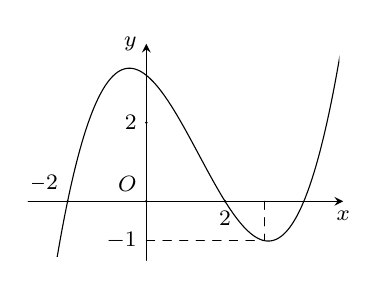
\begin{tikzpicture}[scale=0.5, font=\footnotesize, line join=round, line cap=round,>=stealth]
			\def\a{0.2}  % Hệ số co dãn
			\def\xmin{-3} \def\xmax{5}
			\def\ymin{-1.5} \def\ymax{4}			
			\draw[->] (\xmin,0)--(\xmax,0) node [below]{$x$};
			\draw[->] (0,\ymin)--(0,\ymax) node [left]{$y$};
			\node at (0,0) [above left]{$O$};
			\clip (\xmin+0.1,\ymin+0.1) rectangle (\xmax-0.1,\ymax-0.1);
			\draw[smooth,samples=300] plot(\x,{\a*((\x+2)*(\x-2)*(\x-4))});
			\draw[dashed](0,-1)node[left]{$-1$}--(3,-1)--(3,0);
			\fill (0,0) circle (1.0pt) (-2,0) circle (1.0pt)node[above left]{$-2$} (2,0) circle (1.0pt)node[below]{$2$} (0,2) circle (1.0pt)node[left]{$2$};
		\end{tikzpicture}
	}
	\loigiai{
		Từ đồ thị hàm số, ta có 
		$$\left|f\left(x^3-3x\right)\right|=\dfrac{3}{2}\Leftrightarrow \hoac{& f\left(x^3-3x\right)=\dfrac{3}{2} \\ & f\left(x^3-3x\right)=-\dfrac{3}{2}} \Leftrightarrow\hoac{& x^3-3x=a\text{ với } -2<a<0\\ &x^3-3x=b\text{ với } 0<b<2\\&x^3-3x=c\text{ với } c>2\\ &x^3-3x=d\text{ với } d<-2.}$$
		Xét hàm số $g(x)=x^3-3x$ với $x\in\mathbb{R}$.\\
		$g'(x)=3x^2-3$, $g'(x)=0\Leftrightarrow\hoac{& x=1 \\ & x=-1.}$\\
		Bảng biến thiên
		\begin{center}
			
\begin{tikzpicture}
				\tkzTabInit[nocadre=false,lgt=1.2,espcl=2.5,deltacl=0.6]
				{$x$ /0.6, $g'(x)$ /0.6, $g(x)$ /2.5}
				{$-\infty$,$-1$,$1$,$+\infty$}
				\tkzTabLine{,+,$0$,-,$0$,+,}
				\tkzTabVar{-/$-\infty$,+/$2$,-/$-2$,+/$+\infty$}
			\end{tikzpicture}
		\end{center}
		Từ bảng biến thiên của hàm số $g(x)$, ta có các phương trình
		$$\hoac{& x^3-3x=a\text{ với } -2<a<0 \text{ có } 3 \text{ nghiệm phân biệt} 
			\\ &x^3-3x=b\text{ với } 0<b<2 \text{ có } 3 \text{ nghiệm phân biệt}
			\\&x^3-3x=c\text{ với } c>2 \text{ có } 1 \text{ nghiệm}
			\\ &x^3-3x=d\text{ với } d<-2 \text{ có } 1 \text{ nghiệm}.}$$
		Vậy phương trình $\left|f\left(x^3-3x\right)\right|=\dfrac{3}{2}$ có $8$ nghiệm.
	}
\end{ex}
\Closesolutionfile{ans}
\begin{indapan}{10}
	{ans/ans-2-GHK1-27-NgoGiaTu-Daklak-21}
\end{indapan}